\documentclass[a4paper, 15pt]{article}
\usepackage[left=0.85in, right=0.85in, top=0.5in, bottom=0.95in]{geometry}
\usepackage[T1]{fontenc}
\usepackage[utf8]{inputenc}
\usepackage[italian]{babel}
\usepackage{easyReview}

% Formattazione del testo
\usepackage{setspace}         % Setting dello spazio\begin{spacing}{0.95}
\setstretch{1.2}
\setlength{\parindent}{0pt}
\raggedbottom
\usepackage[none]{hyphenat}    % no sillabazione 
\usepackage{multicol}          % testo su più colonne
\usepackage{changepage}	       % \begin{adjustwidth}{}{}

% Matematica
\usepackage{amsmath, amssymb, amsthm, mathtools}
\usepackage{cancel}            % semplificazioni \cancel{expression}
\newtheorem*{thm}{Teorema}
\newtheorem*{en}{Enunciato}
\newtheorem*{definizione}{Definizione}
\newtheorem*{cor}{Corollario}
\DeclareMathOperator{\rk}{rk}
\DeclareMathOperator{\im}{Im}
\DeclareMathOperator{\ev}{ev}

% Simboli e Disegni
\usepackage{color}             % \textcolor{'ColorCode'}{'testo'}
\usepackage{graphicx, wrapfig, float}
\usepackage{fancyhdr}
\usepackage{tikz, circuitikz}
\usetikzlibrary{patterns, arrows, decorations.markings, arrows.meta, decorations.text}
\tikzset{immagine/.style={above right, inner sep=0pt, outer sep=0pt},
testo/.style={fill=white, align=center, fill opacity=0.6, text opacity=1, below, font=\sffamily\bfseries\footnotesize}}
\usepackage{pgfplots}
\pgfplotsset{compat=1.15}
\usepackage{mathrsfs}

% Altri pacchetti
\usepackage{enumitem}
\usepackage{mdwlist} 	       % suspend enumerate \suspend{} \resume{}
\usepackage{siunitx}
\usepackage{hyperref}
\hypersetup{
colorlinks=true,
linkcolor=blue,    
urlcolor=blue,
}
\urlstyle{same}

% Altre definizioni personali
\usepackage{pifont}
\newcommand{\cmark}{\ding{51}}
\newcommand{\xmark}{\ding{55}}
\DeclareUnicodeCharacter{20AC}{\EUR}
\newcommand{\compresslist}{\setlength{\itemsep}{1pt}\setlength{\parskip}{0pt}\setlength{\parsep}{0pt}}
\newcommand{\ra}[1]{\renewcommand{\arraystretch}{#1}} % stretcho le tabelle e gli array \ra{x}
\setlength{\jot}{10pt}

%=======HEADER & FOOTER=======%
\def\lesson{Lezione N.28}


\pagestyle{fancy}
\fancyhf{}
\renewcommand{\headrulewidth}{0pt}
\renewcommand{\footrulewidth}{1.4pt}
\lfoot{A.M. $\diamond$ \the\year}
\cfoot{\thepage}
\rfoot{\lesson}


% Titolo e data
\title{Parte 21: molle}
\date{}

\begin{document}
\maketitle
\setcounterpageref{secnumdepth}{0}
\setcounter{tocdepth}{5}  % Includo nel TOC anche i subsubpar	
\tableofcontents 
\newpage



%\end{adjustwidth}
%\newpage
\section{Molle}
\begin{adjustwidth}{2in}{}
	La molla è quell'elemento che accumula energia in deformazione elastica ed è in grado di rilasciarla in modo reversibile alla rimozione del carico. 
	
	Per cui l'applicazione delle molle è piuttosto estesa: si possono avere elementi di riportino in posizione meccanismi a seguito di sollecitazioni oppure elementi che vincolino impianti di piping, oppure ancora elementi atti a garantire una certa metodologia di funzionamento. \newline 
	
	Essendo un elemento che deve avere un comportamento reversibile, deve comportarsi  sempre e comunque in modo elastico, per cui quello che deve garantire una molla è l'immagazzinamento di tanta energia di deformazione elastica senza arriva a snervamento. \newline 
	
	La forma della molla garantisce tutto questo. 
	
	Una molla è un qualsiasi oggetto meccanico in grado di assorbire una grande quantità di energia elastica di deformazione, per cui il suo dimensionamento seguirà l'idea di determinazione di una freccia che rapportata al carico necessario per ottenerla darà una rigidezza ed una resistenza opportuna al di  sotto del limite di snervamento. \newline
	
	Gli oggetti come le molle, proprio per la loro funzionalità, sono soggetti a carichi cicli e quindi da dover dimensionare anche a fatica. \newline 
	
	Le molle si classificano sia in funzione della sollecitazione principale che le porta a deformarsi, sia in funzione di un coefficiente di utilizzazione, questo rapporto tra l'energia elastica effettivamente immagazzinata dalla  molla a seguito del carico esterno applicato e la massima energia elastica che quella molla potrebbe immagazzinare se si fosse raggiunto il limite di snervamento su tutti i punti del materiale
	\[C_u = \dfrac{E_e}{E_{\max}}\]
\end{adjustwidth}
\newpage
\subsection{Molle di flessione}
\begin{adjustwidth}{2in}{}	
	Il concetto di molla di flessione più semplice possibile è quello di trave incastrata all'estremo. 
	\begin{figure}[H]
		\centering
		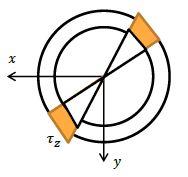
\includegraphics[width=0.5\linewidth]{figures/screenshot001}
		\label{fig:screenshot001}
	\end{figure}
	La trave a mensola si inflette generando uno spostamento a seguito di un carico applicato all'estremità trasversale al piano della molla. \newline
	
	Il coefficiente di utilizzazione sarà pari a 
	\[C_u = \dfrac{{1\over2}Ff}{{1\over2}\dfrac{\sigma^2}{E}V}\]
	Dove le grandezze in gioco - per uno stato di tensione unidirezionale e per una trave a sezione costante - sono 
	\[f = \dfrac{FL^3}{3EI}\qquad I = \dfrac{bh^3}{12}\qquad V = bhL\qquad \sigma = \dfrac{6PL}{bh^2}\]
	Per cui
	\[C_u = {1\over9}\]
	Il coefficiente di utilizzo è molto basso. 
	
	L'andamento delle tensioni è a farfalla e carica al massimo soltanto le fibre orizzontali dell'incastro. 
\end{adjustwidth}
\newpage
\subsection{Molle di torsione}
\begin{adjustwidth}{2in}{}
	La molla di torsione sfrutta, per mezzo di una leva, un momento torcente alle estremità 	attraverso l'indeformabilità a torsione della molla. 
	\begin{figure}[H]
		\centering
		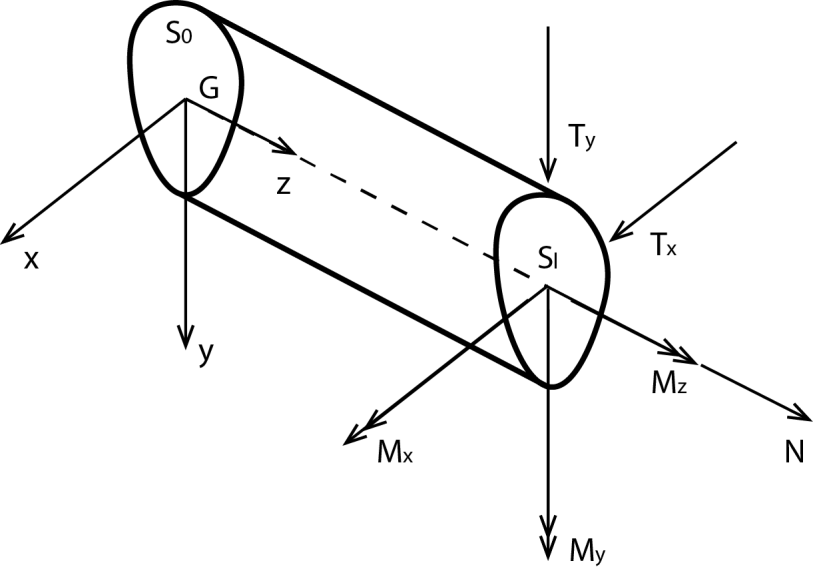
\includegraphics[width=0.5\linewidth]{figures/screenshot002}
		\label{fig:screenshot002}
	\end{figure}
	Solitamente sono barre di torsione. 
	
	In un'autovettura le barre di torsione legano tra loro i ponti posteriori, ovvero i punti di attacco delle sospensioni al fine di evitare il rollio, ovvero la rotazione della vettura durante la percorrenza in curva a seguito del trasferimento di carico che porta ad un affetto centrifugo, si utilizzano queste barre che impongono una resistenza dovuta alla torsione differenziale delle sospensioni. \newline 
	
	Il coefficiente di utilizzazione sarà pari a 
	\[C_u = \dfrac{{1\over2}M\theta}{{1\over2}\dfrac{\tau^2}{V}V}\]
	Dove le grandezze in gioco sono 
	\[\theta = \dfrac{PRL}{GJ}\qquad J = \dfrac{\pi d^4}{32}\qquad V = \dfrac{\pi d^2L}{4}\qquad \tau = \dfrac{16PR}{\pi d^3}\]
	Per cui
	\[C_u = {1\over2}\]
	Il coefficiente di utilizzo è intermedio. 
\end{adjustwidth}
\newpage
\subsection{Molle di trazione}
\begin{adjustwidth}{2in}{}
	Una molla di trazione è semplicemente una trave caricata assialmente a trazione. 	
	\begin{figure}[H]
		\centering
		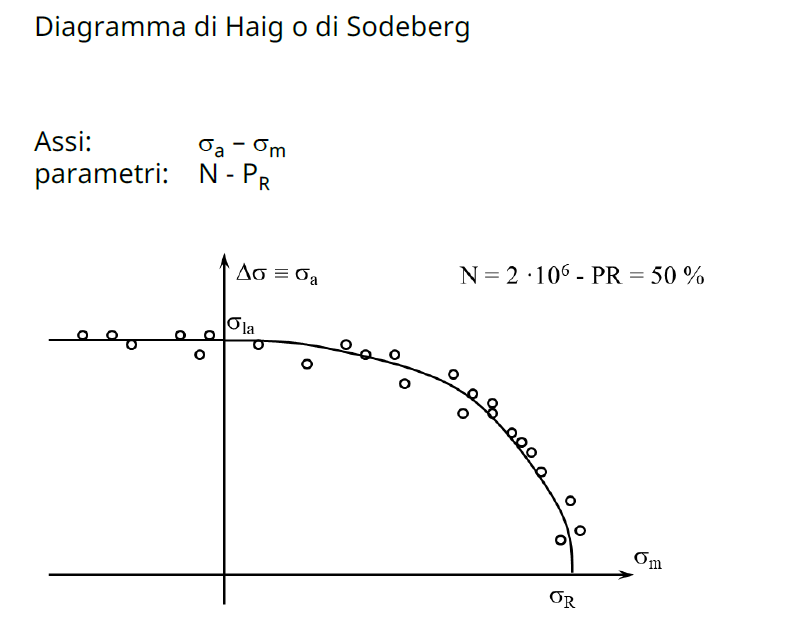
\includegraphics[width=0.2\linewidth]{figures/screenshot003}
		\label{fig:screenshot003}
	\end{figure}
	In questo caso il coefficiente di utilizzazione è pari a 
	\[C_u = \dfrac{{1\over2}Pf}{{1\over2}\dfrac{\sigma^2}{E}V}\]
	Dove le grandezze in gioco sono 
	\[f = \dfrac{PL}{EA}\qquad A = \dfrac{\pi d^2}{4}\qquad V = \dfrac{\pi d^2L}{4}\qquad \sigma = \dfrac{4P}{\pi d^2}\]
	Per cui
	\[C_u = 1\]
	Il coefficiente di utilizzo è massimo. 
	
	Applicando un carico $P$ di trazione si sta uniformemente caricando tutto il materiale: tutti i punti di una sezione in tutte le sezioni. \newline 
	
	la molla di trazione sembrerebbe così la soluzione ideale grazie al coefficiente di utilizzazione unitario. 
	
	Il problema è che la freccia in seguito all'applicazione del carico è molto piccola, comportando una rigidezza enorme. 
	
	Le molle di torsione sfruttano si al massimo il materiale ma sono troppo rigide per le applicazioni reali. (si immagini di sostituire una molla ad elica di un'autovettura con una trave piena...)\newline 
	
	Solitamente si utilizzano o molle di flessione o di trazione. 
\end{adjustwidth}
\newpage
\section{Progetto delle molle}
\begin{adjustwidth}{2in}{}	
	Una molla deve lavorare nelle condizioni che le garantiscano una rigidezza opportuna e al contempo deve resistere alle sollecitazioni statiche e di fatica. 
	
	Le condizioni di verifica strutturale a resistenza sono le medesime di qualunque elemento meccanico (DSV), per cui l'attenzione si focalizzerà sull'elemento funzionale ovvero sulla garanzia di funzionamento. \newline
	
	A seconda dell'applicazione si avrà come richiesta di progetto una determinata rigidezza (sospensioni), una condizione sulla freccia (valvole) o una condizione sulla frequenza (riduzione/generazione vibrazioni), per cui le condizioni funzionali da imporre sono 
	\begin{enumerate}
		\item Condizione sulla freccia 
		\[f = \dfrac{P}{k}\]
		
		\item Condizione sulla frequenza 
		\[\nu = \dfrac{1}{2\pi}\sqrt{\dfrac{k}{m}}\]
	\end{enumerate}
	Per far sì che si possa immagazzinare tanta energia di deformazione elastica senza raggiungere il limite di snervamento, il materiale dovrà avere alto valore di snervamento ed alta deformabilità elastica, si utilizzeranno quindi acciai dall'alto tenore di carbonio (0.6$\div$1.1)\%. 
	
	Si utilizzano anche acciai legati (con leganti non oltre il 5\%) per migliorare soprattutto il funzionamento a fatica, per quanto riguarda la corrosione vengono effettuati opportuni trattamenti superficiali . 
\end{adjustwidth}
%\newpage
\subsection{Molle di flessione}
\begin{adjustwidth}{2in}{}	
Il valore di rigidezza $k$ può essere estratto dalla relazione sulla freccia così come dalla relazione sulla frequenza. 		
\begin{figure}[H]
	\centering
	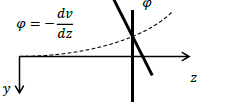
\includegraphics[width=0.5\linewidth]{figures/screenshot004}
	\label{fig:screenshot004}
\end{figure}	
Ponendosi nel caso più semplice possibile, le incognite di progetto sono $L, b, h$. 

Le uniche relazioni utile a fini di progetto sono
\[\sigma = \dfrac{6PL}{bh^2}\leq\sigma_0 \qquad f = \dfrac{PL^3}{3EI} = \dfrac{4PL^3}{Ebh^3}\]
Il problema non si risolve però con 2 relazioni in 3 incognite, questo quindi è un caso in cui il progettista può muoversi abbastanza liberamente scegliendo una terna che soddisfi le due condizioni e che minimizzi altri fattori come volumi, superfici, costi...\newline 

Il problema è che usare una singola lamina come quella in figura per applicazioni reali è piuttosto raro, considerando poi che il coefficiente di utilizzazione è pari a $1\over9$, c'è tanto materiale sotto-sfruttato. \newline 

Per sfruttare maggiormente il materiale si gioca sulla sezione resistente mantenendo il rapporto tra M ed I costante.

In un caso si può ridurre la larghezza, lo spessore od entrambi contemporaneamente.  \newline 

Il caso più semplice è quello di lamina tagliata in larghezza.
\begin{figure}[H]
	\centering
	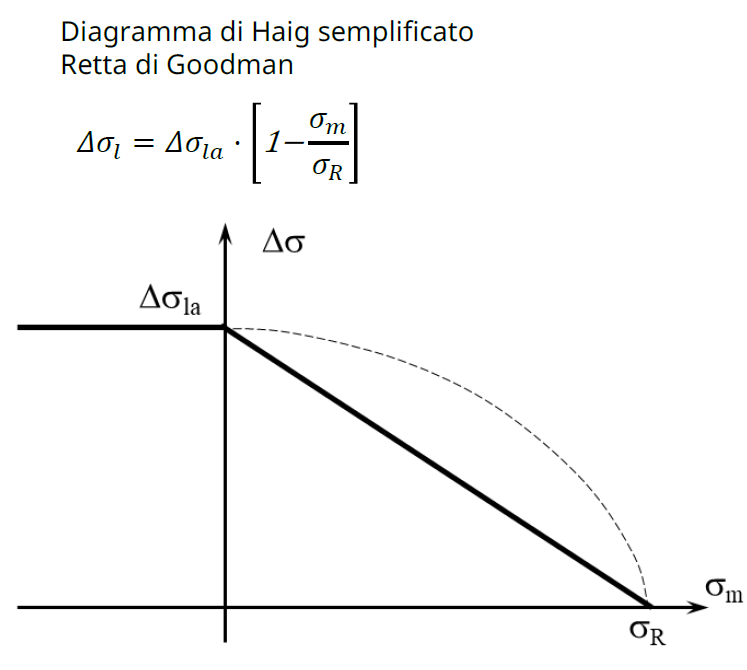
\includegraphics[width=0.5\linewidth]{figures/screenshot005}
	\label{fig:screenshot005}
\end{figure}
Tale larghezza diventa una funzione lineare dell'ascissa curvilinea 
\[b = \dfrac{b_0}{L}x\]
E quindi 
\[\sigma = \dfrac{6Px}{\dfrac{b_0}{L}xh^2} = \dfrac{6PL}{b_0h^2}\]
Che porta a 
\[C_u = {1\over3}\]
È in questo modo aumentato il coefficiente di utilizzazione. 

Se si è in grado di tarare la sezione in modo da avere un rapporto 
\[\dfrac{M}{EI} = \text{cost}\]
Allora vuol dire che si è di fronte ad una linea media che si inflette con curvatura costante proprio pari ad ${1\over R} = {M\over EI}$ e quindi secondo un arco di cerchio. 

Tuttavia nella pratica costruttiva quell'unico punto di applicazione del carico è di scarsa affidabilità, per cui si sceglie una forma più del tipo trapezoidale
\begin{figure}[H]
	\centering
	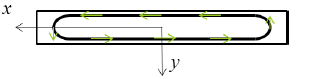
\includegraphics[width=0.5\linewidth]{figures/screenshot006}
	\label{fig:screenshot006}
\end{figure}
la condizione sulla resistenza rimane la medesima (la tensione massima è SEMPRE alla sezione dell'incastro), ciò che cambia  sarà la freccia massima dato che cambia la rigidezza del sistema, con una relazione del tipo
\[f = \dfrac{4KPL^3}{EBh^3} \qquad K = \dfrac{3}{2+\beta}\]
Il principale vantaggio della lamina trapezoidale risiede  nell'ingombro laterale della molla, è necessario molto spazio per alloggiare una molla come quella in figura. \newline 

Per soprassedere a questo problema si taglia la lamiera così dimensionata.
\begin{figure}[H]
	\centering
	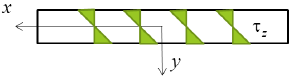
\includegraphics[width=0.7\linewidth]{figures/screenshot007}
	\label{fig:screenshot007}
\end{figure}
Queste foglie vengono così sovrapposte l'una con l'altra ottenendo una \textbf{molla a balestra}.
\begin{figure}[H]
	\centering
	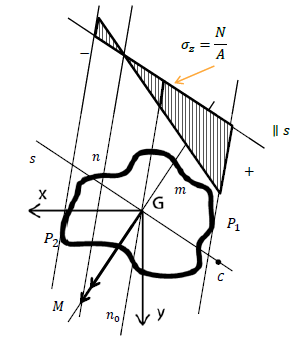
\includegraphics[width=0.7\linewidth]{figures/screenshot008}
	\label{fig:screenshot008}
\end{figure}
Una volta realizzata la lamina triangolare si tagliano delle \textit{foglie} e si sovrappongono l'una sull'altra. 

In questo modo si ottiene un oggetto molto meno ingombrante il larghezza, un po' più ingombrante in spessore e dalle prestazioni analoghe a quelle della lamiera madre. 

Il sistema prevede un ancoraggio alle estremità mediante cerniera-carrello con  il punto di applicazione della forza in mezzeria. 

A differenza del sistema originario questo è un sistema appoggio-appoggio, tuttavia essendo il punto di applicazione della forza mediano, sfruttando la simmetria è come se si avesse un incastro ed un estremo libero assimilando tale tale ad una lamina incastrata usando la metà della luce tra gli appoggi. \newline 

Nella realtà una molla a balestra lavora con delle complessità aggiuntive: le foglie  possono non essere tutte perfettamente planari, possono esserci degli scorrimenti tra le foglie se non delle deformazioni fuori dal piano. 

Il comportamento reale di questo tipo di molla non è perfettamente reversibile, ma è sempre isteretico. 

Nella pratica la balestra è precaricata, viene cioè montata con  linea media arcuata, in questo modo c'è un precarico assiale sul materiale applicato tra l'altro con una inclinazione $\alpha$ in modo da avere anche una componente di taglio, in questo modo oltre ad avere l'inflessione tipica dovuta al carico $P$ ortogonale, ci sarà anche una componente di momento flettente locale ed una componente di compressione assiale, sempre al fine di sfruttare il più possibile il materiale. 
\begin{figure}[H]
	\centering
	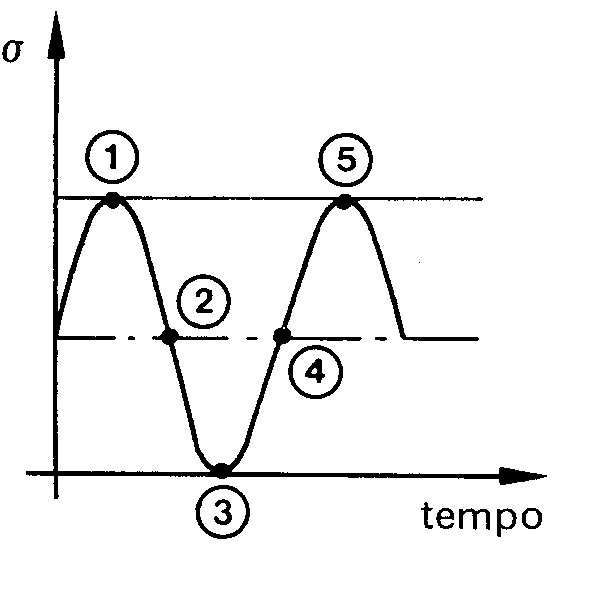
\includegraphics[width=0.7\linewidth]{figures/screenshot009}
	\label{fig:screenshot009}
\end{figure}
In questa configurazione l'inflessione che si va a generare è più complessa da ricavare. 
\[f = K\dfrac{4PL^3}{Enb_1h^3}\left(1+1,3\dfrac{c}{l}\tan\alpha\right)\]
Le relazioni di verifica si basano contemporaneamente sugli approcci funzionale e di resistenza 
\[f = K\dfrac{4PL^3}{Enb_1h^3} \qquad \sigma = \dfrac{6PL}{nb_1h^2}\]
In queste relazioni le incognite diventano però 4, oltre ad $L, h, b_1$ si aggiunge $n$ numero di foglie necessarie. 

Tuttavia anche in questo caso, fissati dei valori per garantire alcune proprietà, si può passare al dimensionamento. 
\end{adjustwidth}
%\newpage
\subsection{Molle di torsione}
\begin{adjustwidth}{2in}{}	
Le molle di torsione hanno un maggior coefficiente di sfruttamento.

La forma caratteristica è sempre la stessa: una trave a sezione circolare (così ho una torsione che non porta a ingobbamento) e viene attivata mediante l'applicazione di un momento torcente, di solito attraverso la conversione di un carico mediante una leva. 
\begin{figure}[H]
	\centering
	\includegraphics[width=0.5\linewidth]{figures/screenshot0010}
	\label{fig:screenshot0010}
\end{figure}
Anche in questo caso le incognite sono tre: $R, d, L$. 
\[\tau = \dfrac{16PR}{\pi d^3}\leq\tau_0 \qquad J = \dfrac{\pi d^4}{32} \qquad f = R\theta = \dfrac{PR^2L}{GJ}\]
Mentre i dati di progetto sono $P, f$. 
\end{adjustwidth}
\newpage
\subsubsection{Molle ad elica}
\begin{adjustwidth}{2in}{}
La molla ad elica non è altro che una molla di torsione che viene deformata lungo un'elicoide: è un filo d'acciaio ripiegato a seguire un'elica. 
\begin{figure}[H]
	\centering
	\includegraphics[width=0.5\linewidth]{figures/screenshot0011}
	\label{fig:screenshot0011}
\end{figure}
L'applicazione del carico in mezzeria al cilindro intorno a quale viene avvolta l'elica, genera sul singolo filo in prevalenza una torsione. \newline 

I parametri da dimensionare sono sicuramente il diametro della sezione circolare del filo $d$, il diametro dell'elica $D$, l'altezza complessiva della molla $h$ e il passo della molla $p$ questo inteso come distanzia assiale che percorre l'elica per fare un giro completo. \newline 

Una molla ad elica è in grado di lavorare a compressione e a trazione, con l'unica distinzione data dal fatto che, se la molla lavora a trazione, il limite è dato dalla resistenza del materiale, fino allo snervamento, a compressione si aggiunge un limite funzionale: lo spostamento masso è limitato  dal numero di spire e dal passo della spira, si può comprimere fino al completo contatto tra le spire (configurazione a pacco); al raggiungimento di questa condizione la rigidezza diventa estremamente più elevata. 

Alle estremità di una molla possono esserci dei tappi, delle superfici per ripartire meglio il carico oppure dei ganci. 

In entrambi i casi si possono distinguere un certo numero di spire libere - quelle che effettivamente lavoreranno durante il funzionamento della molla - e un certo numero di spire morte, come quelle magari alloggiate sui tappi, che non compiono lavoro di deformazione. \newline 

È molto importante quantificare il passo al fine di evitare la configurazione a battuta della molla, generalmente questo viene posto costante anche se in alcune applicazioni possono essere utili molle a passo variabile. 

La differenza tra i due tipi di molle sta tutto nel loro lavoro durante la compressione, se col passo costante la rigidezza è costante fino alla battuta, col passo variabile le spire con un passo minore cominciano a toccarsi tra loro facendo variare la rigidezza della molla, variando linearmente con la quantità di spire che si sta toccando caratterizzando nell'insieme uno spostamento non lineare (quadratico).  \newline 

Rispetto alla classica barra di torsione rettilinea il materiale è sollecitato in modo più complesso: mentre la barra lineare aveva una carico applicato ad una certa distanza $R$, in questo caso la sollecitazione che si applica su una sezione dipende dal fatto che il carico applicato genera, oltre che a un taglio ed un momento torcente (proprio come nella barra di torsione originaria), anche una forza trasversale all'elica e una forza allineata all'elica. 

Dato che è applicato su un elemento che oltre ad essere di rivoluzione segue anche un'elica avendo un asse inclinato di un certo angolo, si avrà la scomposizione del carico $P$ in una forza trasversale all'elica e una forza allineata all'elica quindi una sollecitazione di taglio e di compressione/trazione assiale. 
\begin{figure}[H]
	\centering
	\includegraphics[width=0.5\linewidth]{figures/screenshot0012}
	\label{fig:screenshot0012}
\end{figure}
Inoltre il vettore momento applicato $\vec{M} = P{D\over2}$ ha una componente  lungo l'asse dell'elica portando ad un momento torcente ed una piccolissima componente di flessione. 

Per cui se è vero che la sollecitazione preponderante è quella di torsione, è anche vero che ci sono anche una sollecitazione di taglio, si trazione/compressione e di flessione. \newline 

Il dimensionamento si fa prevalentemente a torsione anche se esistono modelli che tengono conto anche delle sollecitazioni aggiuntive. 

Il coefficiente che distingue una barra di torsione da una molla ad elica è il rapporto $C$ fra il diametro d'elica ed il diametro del filo. 

Nel caso della barra di torsione $C\rightarrow\infty$: è come se si avesse un'elica a diametro infinito. 

Le differenze di freccia sono paragonabili in termini di rotazione, si possono allora utilizzare le frecce in mezzeria esattamente come era stato fatto con la barra di torsione.

All'estremità della barra di torsione si leggeva uno spostamento $f$ dettato dalla lunghezza della leva $R$ per la rotazione della sezione $\theta$, analogamente la freccia dell'elica è data da 
\[f=R\theta = \dfrac{32PR^2L}{G\pi d^4}\]
Per valutare le correzione aggiuntive allo stato tensionale si può utilizzare, secondo Wahl, un coefficiente 
\[\lambda_\tau = \dfrac{4C-1}{4C-4} + \dfrac{0.615}{C}\]
Una molla di questo tipo si dimensiona sempre a partire dalla scelta del materiale dalla giusta tensione ammissibile tenendosi sempre un certo margine dovuto alla concentrazione di tensione 
\[k_t = \lambda_\tau\]
Si assume poi un valore di diametro del filo, scelto a partire da valori commerciali e ci si trova i valori di diametro $D$ ed $L$ in funzione delle relazioni funzionali  viste nella barra di torsione. 

Dopodiché si sceglie un angolo d'elica $\alpha$ e si calcola il passo
\[p = \pi D\tan\alpha\]
L'altezza totale della molla sarà dato da 
\[H = np + n_md\]
Dove $n$ è il numero di spire attive ed $n_m$ è il numero di spire morte. 

A questo punto ci si trova un sistema di equazioni in cui la condizione di scelta dei diametri e delle lunghezze è dettata dagli ingombri 
\[D<D_{\max} \qquad H<H_{\max}\]
La condizione sull'altezza minima invece è quella di non mandare a battura la molla
\[H-f >(n+n_m)d\]
Una volta fissate le geometrie è possibile ricavarsi il fattore di concentrazione delle tensioni ed utilizzarlo all'interno delle formule per le verifiche resistenziali. \newline 

La condizione a battuta porta ad aver un carico massimo  da NON raggiungere, cioè associato a quello spostamento massimo ci sarà un carico massimo. 
\[f_{\max} = H - (n+n_m)d \qquad P_{\max} = \dfrac{f_{\max}G\pi d^4}{32R^2L}\]
Un'altra condizione da dover verificare è quella sull'instabilità. 

Molto spesso, prima di portare a battuta una molla dalle piccole dimensioni (penna a scatto), questa si inflette in una direzione causando un'eccentricità, si è verificato il fenomeno dell'instabilità euleriana; questa infatti incorre nelle molle per livelli di carico estremamente bassi. 

In sostanza i valori di compressione massimi di una molla sono molto differenti in funzione delle condizioni di vincolo. 
\end{adjustwidth}
\newpage
\section{Sistemi di molle}
\begin{adjustwidth}{2in}{}
	Molto spesso l'applicazione non sarà della singola molla ma di una certa quantità di molle in serie o in parallelo. 
	
	Per motivi di semplicità grafica molto spesso si ragiona su questi tipi di molle utilizzando le molle ad elica, tuttavia discorso è facilmente estendibile a qualsiasi sistema strutturale lavorando a parametri concentrati.  	
	\begin{figure}[H]
		\centering
		\includegraphics[width=0.5\linewidth]{figures/screenshot0013}
		\label{fig:screenshot0013}
	\end{figure}
	Lavorando sulla rigidezza singole molle in questo modo, si può ottenere la rigidezza equivalente voluta. 
	
	Per due molle in serie lo spostamento totale è pari a 
	\[f_{tot} = f_1 + f_2 \]
	Poiché gli spostamenti sono pari $ f = {F\over k}$, dato che la forza che subiscono le molle è la stessa, si ottiene che due molle in serie hanno una rigidezza equivalente pari a 
	\[\dfrac{1}{k_{eq}} = \dfrac{1}{k_1} +\dfrac{1}{k_2}\]
	
	Se le molle invece sono in parallelo, all'applicazione del carico c'è una ripartizione 
	\[F_{tot} = F_1 + F_2\]
	Ciascuna molla tuttavia si abbassa della stessa quantità, per cui 
	\[k_{eq} = k_1+k_2\]
	Per ricavare un sistema non lineare, oltre a lavorare sul passo dell'elica, si può modificare la disposizione della specifica elica, e quindi in alcuni casi si decide di lavorare con delle molle che si attivino in particolari condizioni usando diverse altezze. 
\begin{figure}[H]
	\centering
	\includegraphics[width=0.2\linewidth]{figures/screenshot0014}
	\label{fig:screenshot0014}
\end{figure}
In questo modo si ottiene un sistema che inizialmente ha la rigidezza della prima molla ed effettuato un determinato spostamento entra in gioco la seconda molla. 

Entrando in gioco la seconda molla, il sistema sarà più rigido, per cui si avrà un contributo ulteriore di rigidezza.  

Similmente, se la seconda molla si attivasse in serie, il sistema sarebbe meno rigido. 

Una delle molla a passo variabile ad esempio, si può facilmente vedere come un sistema di molle in serie, dove ciascuna elica concorre ad essere una molla, a mano a mano che va a battuta la rigidezza diviene infinita ed il sistema diventa sempre più rigido. 
































\newpage
\textbf{{\LARGE NOTE}}
%	\vfill
%	\begin{tcolorbox}[height=4.5cm]
%		This box has a height of 4.5cm.
%	\end{tcolorbox}

%DA DECOMMENTARE PER AVERE LA VERSIONE STAMPABILE A DUE PAGINE 	
%	\newpage
%		\null
%		\vfill
%\begin{tcolorbox}[height=4.5cm]
%	This box has a height of 4.5cm.
%\end{tcolorbox}
%		
\end{adjustwidth}
\end{document}